\documentclass[12pt]{article}

\usepackage{xeCJK}%字體設定
\setCJKmainfont{cwTeXKai}[AutoFakeBold=1.5]


\setmainfont{Times New Roman}  % 英文正文字體

\usepackage[top=2cm,bottom=2cm,left=2cm,right=2cm,a4paper]{geometry}%版面設定

\usepackage{indentfirst}%縮排

\usepackage{setspace}%行距設計
\onehalfspacing%半行距
\setlength{\parskip}{3pt}%段落之間

\usepackage{moresize}%字體大小

\usepackage{graphicx}

\usepackage{amssymb}%數學符號

\usepackage{amsmath} % 數學符號
\usepackage{booktabs}         % 漂亮的表格（\toprule, \midrule, \bottomrule）
\usepackage{siunitx}          % 國際單位制 (建議處理單位更漂亮)

\usepackage{multicol}%引入函數使下面那些可以變成雙欄

\usepackage{float}%圖片固定

\usepackage{subcaption}

% --- 程式碼樣式 ---
% 設定 listings 用的字體
\usepackage{listings}          % 插入程式碼
\usepackage{xcolor}            % 程式碼顏色
\setmonofont{Courier New} % 設定等寬字體
\lstset{
  basicstyle=\ttfamily\small, % 使用等寬字體顯示程式碼
  numbers=left,
  numberstyle=\tiny,
  keywordstyle=\color{blue},
  commentstyle=\color{green!50!black},
  stringstyle=\color{red},
  breaklines=true,
  frame=single,
  tabsize=2,
  showspaces=false,      % 不要把空格顯示成 ␣
  showstringspaces=false % 不要在字串裡顯示 ␣
}

% \renewcommand{\thesection}{\Roman{section}}


%%%%%%%%%%%%%%%%%%%%%%%%%%%%%%正文%%%%%%%%%%%%%%%%%%%%%%%%%%%%%%%%%%%
\begin{document}

\begin{titlepage}
\begin{center}

\vspace*{0.5cm}
\HUGE \textbf{普通物理實驗結報}\\
\vspace{4cm}
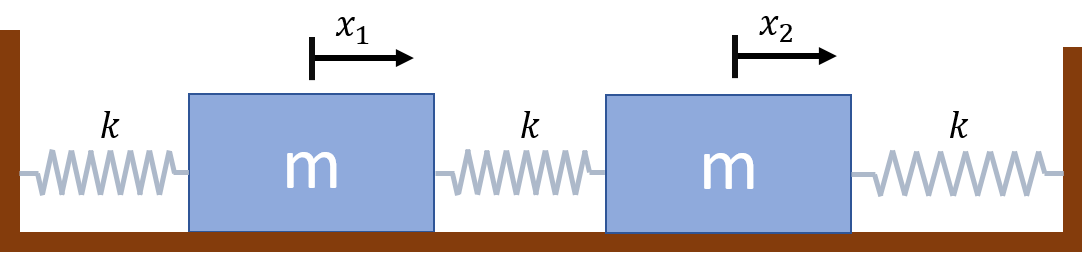
\includegraphics[width=15cm]{IMG_0412.png}\\[2cm]
\HUGE \textbf{耦合振盪}\\

\vfill
\huge 第三組\\[0.5cm]
\begin{table}[h]
\centering
\Large
\begin{tabular}{|c|c|}
\hline
組員:              & 貢獻度  \\
吳 & 37.5\% \\
卓& 37.5\% \\
程& 25\% \\ \hline
\end{tabular}
\end{table}

\end{center}

\end{titlepage}

%%%%%%%%%%%%%%%%%%%%%%%%%%%%%%%%%%%%%%%%%%%%%%%%%%%%%%%%%%%%%%%%

\large
\section{\textbf{實驗目的}}
在這次實驗， 我們有幾個關鍵目的：
    \begin{enumerate}
        \item 透過實驗觀察耦合振盪的整體行為與其各種動態特性，並深入理解系統中能量在振子之間傳遞的方式。
        \item 利用 \textbf{\textit{Python}} 程式進行耦合振盪系統的數值模擬，將模擬結果與實際實驗觀察進行對照與分析，以驗證模型的準確性與可用性。
        \item 探討並學習不同參數（如初始條件、摩擦、彈簧常數等）的改變對耦合振盪系統造成的影響，從而加深對物理機制與系統敏感度的理解。
    \end{enumerate}
%%%%%%%%%%%%%%%%%%%%%%%%%%%%%%%%%%%%%%%%%%%%%%%%%%%%%%%%%%%%%%%%
\section{\textbf{實驗原理}}
考慮兩個相同質量、以彈簧連接的耦合震盪系統：兩端各有彈性常數為 $k$ 的彈簧連接在固定牆面，兩質點之間以彈簧常數為 $k_c$ 的彈簧連接。令兩質點的位移分別為 $x_1(t)$ 與 $x_2(t)$，且向右為正。
\noindent
由受力平衡可寫出兩運動方程：
\begin{align}
m\ddot{x}_1 &= -k x_1 - k_c(x_1 - x_2), \label{eq:motion1} \\
m\ddot{x}_2 &= -k x_2 - k_c(x_2 - x_1). \label{eq:motion2}
\end{align}
整理方程式成矩陣形式的聯立方程式：
\[
m
\begin{pmatrix}
\ddot{x}_1 \\[6pt]
\ddot{x}_2
\end{pmatrix}
+
\begin{pmatrix}
k + k_c & -k_c \\[6pt]
-k_c & k + k_c
\end{pmatrix}
\begin{pmatrix}
x_1 \\[6pt]
x_2
\end{pmatrix}
= 0
\]
\noindent
簡化後定義矩陣
\[
\mathbf{A} =
\begin{pmatrix}
k + k_c & -k_c \\
-k_c & k + k_c
\end{pmatrix},
\qquad
\mathbf{x}(t) = \begin{pmatrix} x_1(t) \\ x_2(t) \end{pmatrix}.
\]
The equations of motion can be expressed as
\[
m\ddot{\mathbf{x}}(t) + \mathbf{A}\,\mathbf{x}(t) = \mathbf{0}
\]


\noindent
求解該系統的震盪模態，我們假設:
\[
\mathbf{x}(t) = \mathbf{B}\,e^{i\omega t},
\qquad \mathbf{B} = \begin{pmatrix} B_1 \\ B_2 \end{pmatrix},
\]
其中 $\omega$ 為角頻率，$\mathbf{B}$ 為對應的震盪模式。將此假設代回運動方程：
\[
\big( \mathbf{A} - m\omega^2 \mathbf{I} \big)\mathbf{B} = \mathbf{0}.
\]
\noindent
非零解 $\mathbf{B}\neq\mathbf{0}$ 的存在條件是矩陣 $\mathbf{A} - m\omega^2 \mathbf{I}$ 的行列式為零，即：
\[
\det\!\big( \mathbf{A} - m\omega^2 \mathbf{I} \big) = 0.
\]
\noindent
求解矩陣$\mathbf{A}$特徵值後:
\[ 
\lambda_1=k ,\lambda_2=tr(A)-\lambda_1=k+k_c
\]
$\because\lambda=m\omega^2$
$\therefore\omega=\sqrt{\frac{\lambda}{m}}$
代入後可得兩種角頻率:
\begin{itemize}
    \item $\omega_1=\sqrt{\frac{k}{m}}$
    \item $\omega_2=\sqrt{\frac{k+2k_c}{m}}$
\end{itemize}

因此系統共有兩個模態對應兩個頻率$\omega_1,\omega_2$。

\section*{兩模態所對應的特徵向量}
\noindent
將特徵值代入 $(\mathbf{A}-m\omega^2\mathbf{I})\mathbf{B}=\mathbf{0}$：

\paragraph{同相 $(\omega=\omega_1)$}

代入 $m\omega_1^2 = k$，矩陣第一行變為
\[
(k+k_c - k)B_1 - k_c B_2 = k_c(B_1 - B_2) = 0,
\]
因此 $B_1 = B_2$，代表兩質點同向移動。特徵向量為 $\mathbf{B_1} = (1,1)^{\mathrm{T}}$。

\paragraph{反相 $(\omega=\omega_2)$}

代入 $m\omega_2^2 = k+2k_c$，第一行變為
\[
(k+k_c - (k+2k_c))B_1 - k_c B_2 = -k_c(B_1 + B_2) = 0,
\]
因此 $B_1 = -B_2$，代表兩質點反向移動。\\
特徵向量為 $\mathbf{B_2} = (1,-1)^{\mathrm{T}}$。
%%%%%%%%%%%%%%%%%%%%%%%%%%%%%%%%%%%%%%%%%%%%%%%%%%%%%%%%%%%%%%
% \section{\textbf{理論分析}}

% 這裡放文字

%%%%%%%%%%%%%%%%%%%%%%%%%%%%%%%%%%%%%%%%%%%%%%%%%%%%%%%%%%%%%%%%

\section{\textbf{實驗方法}}
建立耦合系統:兩個彈簧-滑車系統，並使用相機結合運動分析軟體:Tracker來記錄和分析運動軌跡,探討頻率、振幅等關係,並用python模擬。
%%%%%%%%%%%%%%%%%%%%%%%%%%%%%%%%%%%%%%%%%%%%%%%%%%%%%%%%%%%%%
In this particular experiment, we will be particularly focus primarily on the \textbf{initial condition }of the setup and the recording of the research object's \textbf{motion data }of two different oscillation behavior (\textit{forms}). The data later will be used for simulation and comparison purposes.

%%%%%%%%%%%%%%%%%%%%%%%%%%%%%%%%%%%%%%%%%%%%%%%%%%%%%%
\subsection{Experiment 1:  the Symmetric Form}
Setup the instrument and make sure everything remains stable and constant. Before starting, the word '\textit{Symmetric}" means \textit{uniformity}, it is a word used for \textit{conformity}. This means that in this part of the experiment, we will be dealing with motion that move in the \textbf{same direction} in the same \textbf{phase} of time. And for data collection, video recording will be done, later to be used for analysis purposes.

They usually have the initial condition as:
\[x_1(0)=x_2(0)\neq0\]
\[v_1(0)=v_2(0)=0\]

\subsection{Experiment 2: the Asymmetric Form}
Unlike before, this part deals with motions completely \textbf{opposite} of \textit{experiment 1}'s motions, which uniformly moves together. Experiment 2 deals with 'uniformless' motion or motions whose direction is not the same at the same phase of time. Meaning, one of the movement vectors may go right at time $t$, but at the same time, they will be also be companied with some other movement vector that moves in a entirely \textit{opposite} direction relative to the first vector. In conclusion, their direction will be \textit{opposite} to one another. For data collection, the same data collection method in \textit{experiment 1 }will be used in this part.

They usually have the initial condition as:
\[x_1(0)=-x_2(0)\neq0\]
\[v_1(0)=v_2(0)=0\]

\subsection{Experiment 3: Video Analysis}
With both data points being collected, analysis will be done with the application '\textit{Tracker}'". It will be mainly used to track the movement of the two conform types of motion forms, in regards to time. \textit{Oscillation frequency }will also be measured in this part.

\subsection{Experiment 4: Simulation using Python}
Simulation will be primarily used to compare our "\textit{Tracker}" analysis results to the supposed theoretical output, given by the \textbf{simulation}.
%%%%%%%%%%%%%%%%%%%%%%%%%%%%%%%%%%%%%%%%%%%%%%%%%%%%%%%%%%%%%%%%

\section{\textbf{數據分析}}
%%%%%%%%%%%%%%%%%%%%%%%%%實驗一%%%%%%%%%%%%
\subsection{實驗一:彈性係數}
\begin{figure}[H]
    \centering
    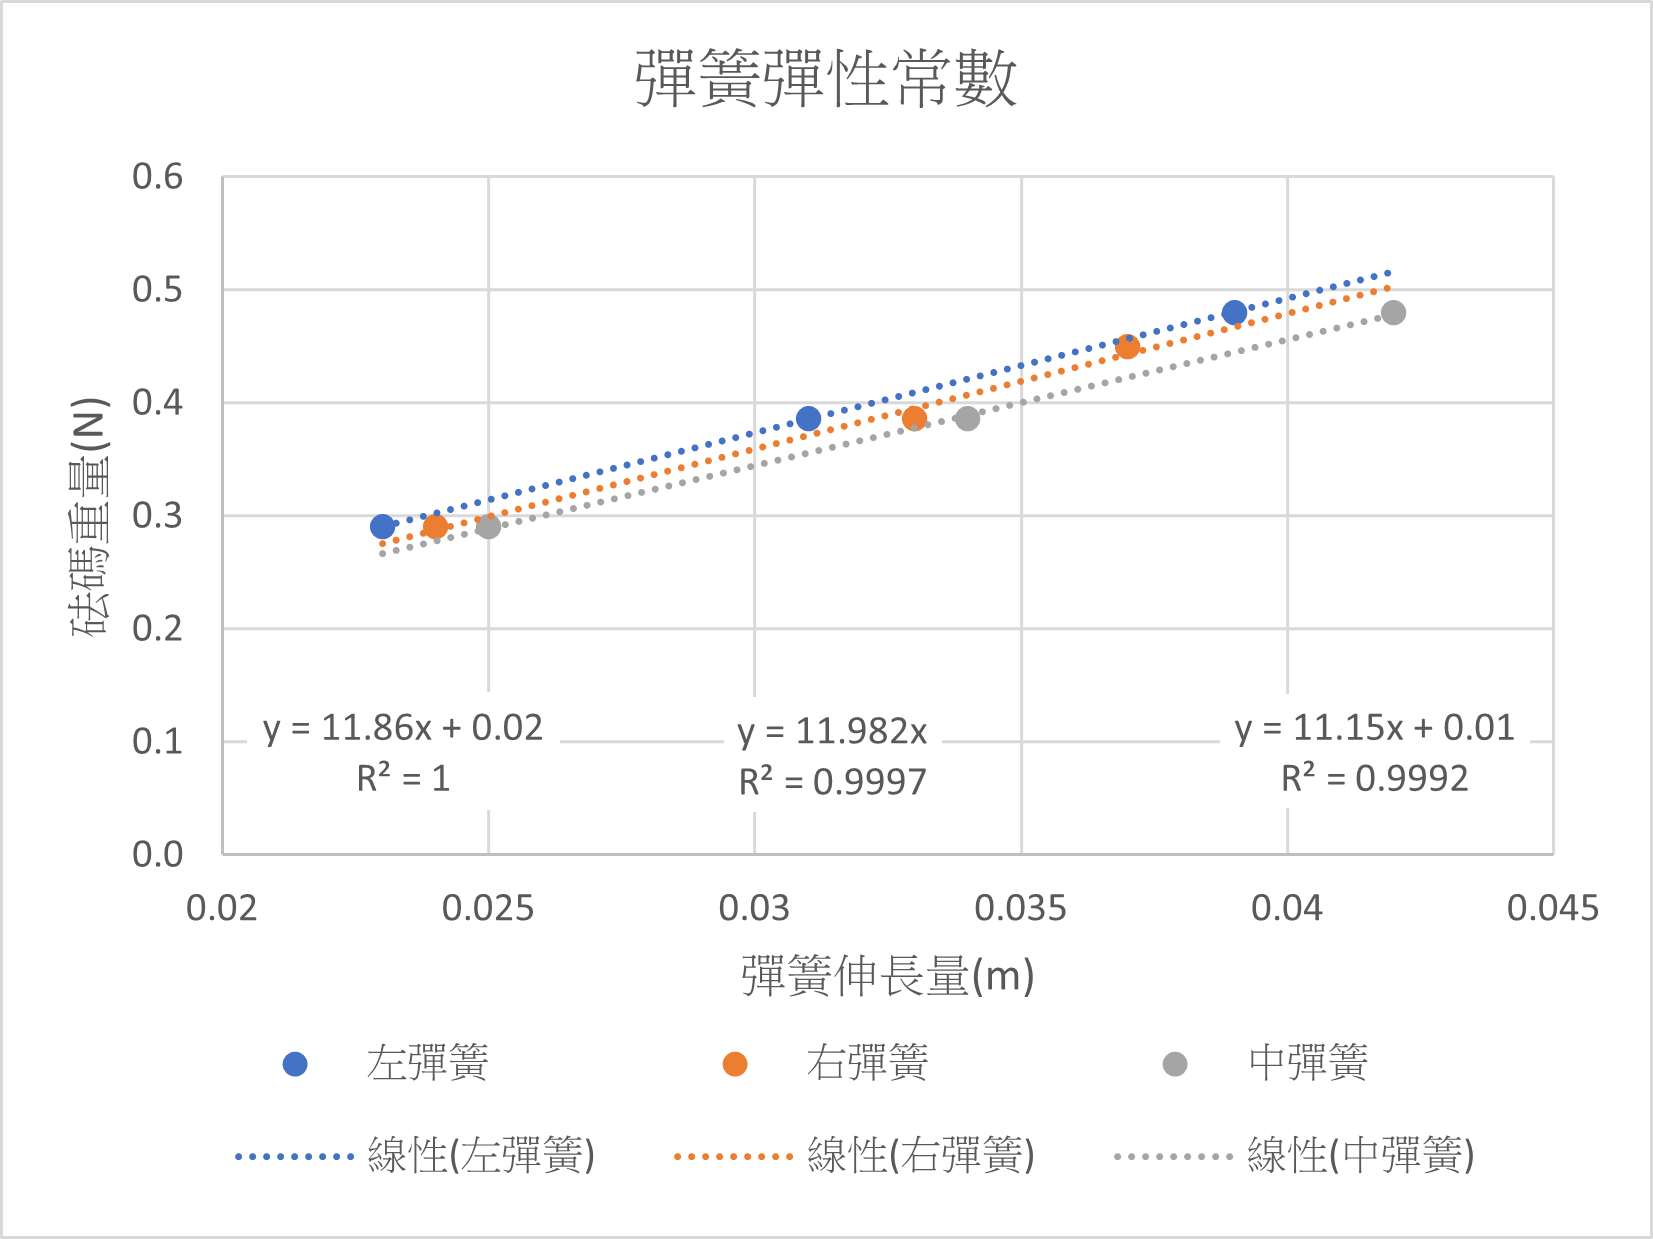
\includegraphics[width=0.8\linewidth]{反向圖表/彈性常數.png}
    \caption{彈性常數}
    \label{fig:彈性常數}
\end{figure}
\noindent
\begin{itemize}
    \item 所測出的彈性系數分別為:$k_1=11.86$(左)，$k_2=11.15$(中)，$k_3=11.98$(右)\\
    \item 理論推導部分有要求左右彈簧的彈性係數需相同，但若我們計算在上述彈性係數的模態與特徵值可得:
\[
\mathbf{A}=
\begin{pmatrix}
   23.01 && 11.15\\
   11.15 && 23.13\\
\end{pmatrix} , \lambda_1\approx11.92 , \lambda_2\approx34.22\\
\]
\[v_1=
\begin{pmatrix}
   -1.018\\
   1\\
\end{pmatrix}
 , v_2=
\begin{pmatrix}
   0.995\\
   1\\
\end{pmatrix}
\]
而若取左右兩彈簧彈性常數平均計算，可得:
\[
\mathbf{A}=
\begin{pmatrix}
   23.07 && 11.15\\
   11.15 && 23.07\\
\end{pmatrix} , \lambda_1=11.92 , \lambda_2=34.22\\
\]
\[v_1=
\begin{pmatrix}
   -1\\
   1\\
\end{pmatrix}
 , v_2=
\begin{pmatrix}
   1\\
   1\\
\end{pmatrix}
\]
因為兩種情形的特徵值相同，所以並不會影響到角頻率的測量，兩者間只會有模態間的差異，不至於產生較大誤差。
\end{itemize}
%%%%%%%%%%%%%%%%%%%%%%%%%%%%%%實驗二%%%%%%%
\subsection{實驗二:同/反向運動的角速度}
\noindent
一維運動所測得動摩擦係數為$\mu=0.002$\\
左邊滑車質量$=0.388kg$，右邊滑車質量$=0.388kg$\\
$\omega=\sqrt{\frac{k}{m}}=5.5 4\ \mathrm{rad/s}$
\subsubsection{\textbf{同向震盪}}
\noindent
初始位置:$x_1=30cm,x_2=60cm$\\
彈簧變化量:$\Delta x_1=0.03cm,\Delta x_2=0.03cm$\\
    \begin{figure}[H]
        \centering
        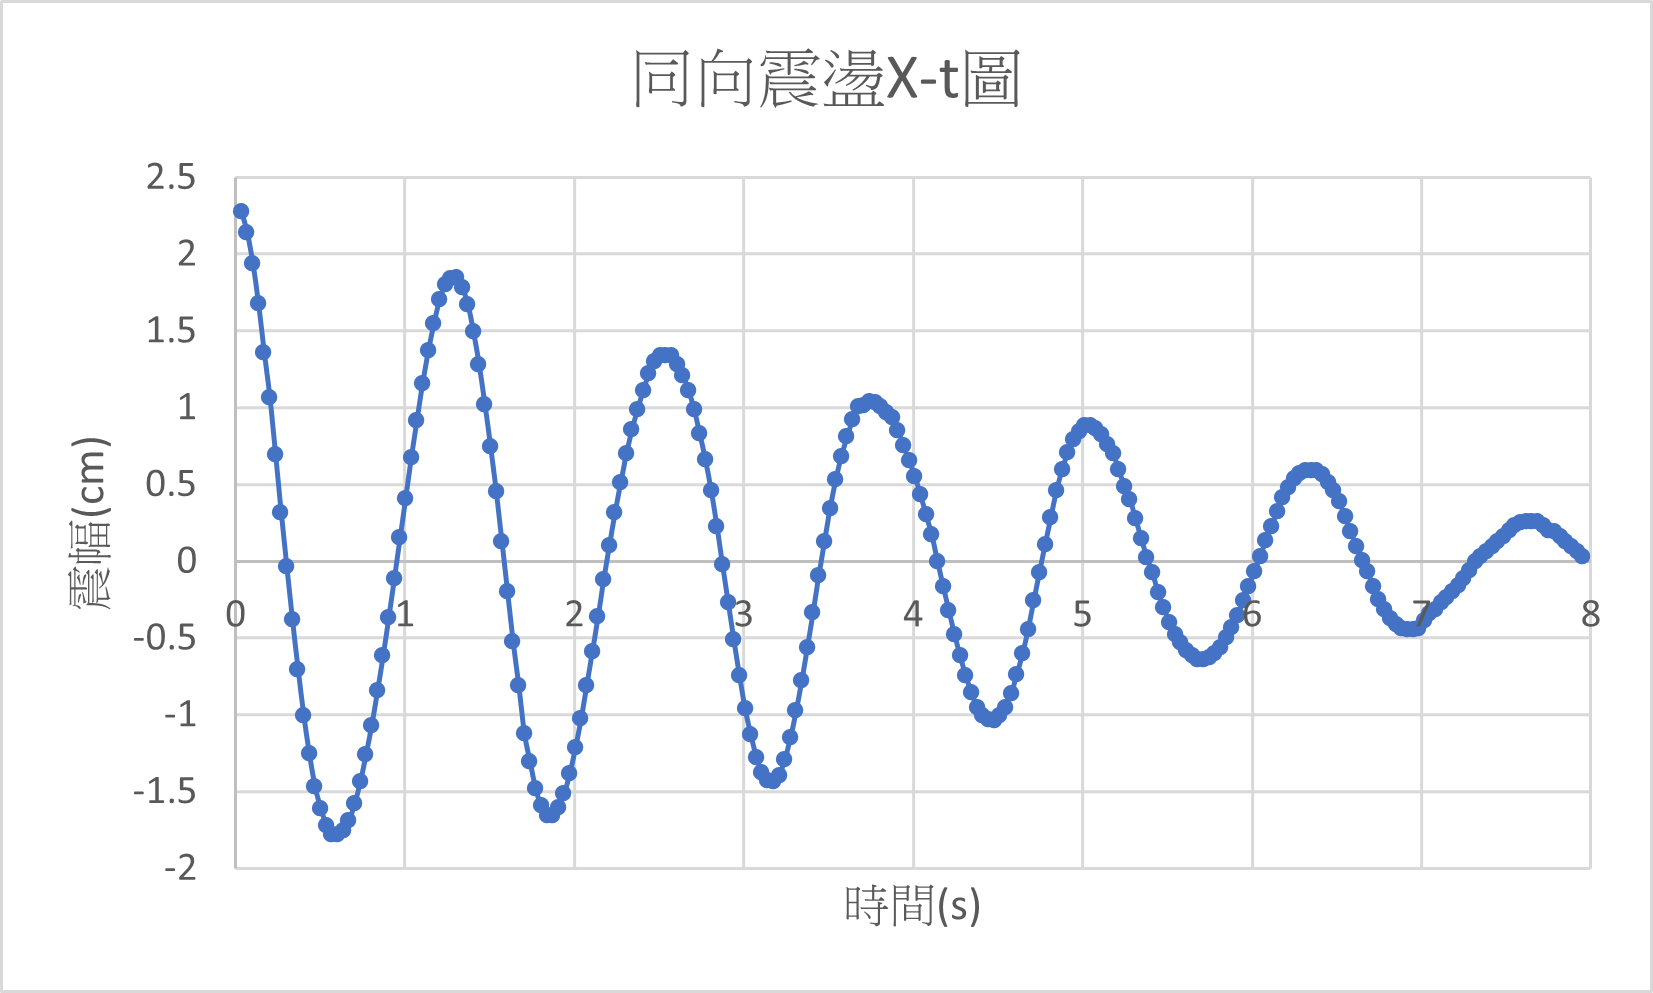
\includegraphics[width=0.7\linewidth]{同向圖表/同向震盪xt圖.png}
        \caption{同向震盪xt圖}
        \label{fig:同向震盪xt圖}
    \end{figure}
以下我們分別透過 C語言、Traker內建之FTT、python分別對實際實驗數據，擬合結果分析角速度之大小:
\begin{enumerate}
    
    \item \textbf{C語言}\\
         我們原本預期使用 C 語言程式自動記錄實驗數據的峰值與時間，但如圖 \ref{fig:同向C} 所示，由於該組實驗數據過少，無法直接進行計算。因此，我們改用手動計算，得到平均週期與對應角速度如下：
        \begin{center}
         $T_{\text{avg}} = 1.261\ \mathrm{s}$ \\
         $\omega_c = 4.98\ \mathrm{rad/s}$
        \end{center}

            \begin{figure}[H]
                \centering
                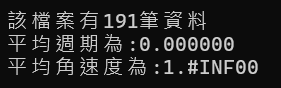
\includegraphics[width=0.5\linewidth]{同向圖表/螢幕擷取畫面 2025-11-23 155611.png}
                \caption{C運行結果}
                \label{fig:同向C}
            \end{figure}
        
    \item \textbf{Traker內建之FTT}\\
        使用 Tracker 內建的快速傅立葉轉換（FFT）功能對實驗數據進行頻域分析。分析結果如圖 \ref{fig:trackerFTT分析結果} 所示。在頻域中，峰值出現在 $f = 0.793$ Hz。根據此頻率，可以計算對應的角速度：
        \[
        \omega_T=2\pi f=4.98\ \mathrm{rad/s}
        \]
    
            \begin{figure}[H]
                \centering
                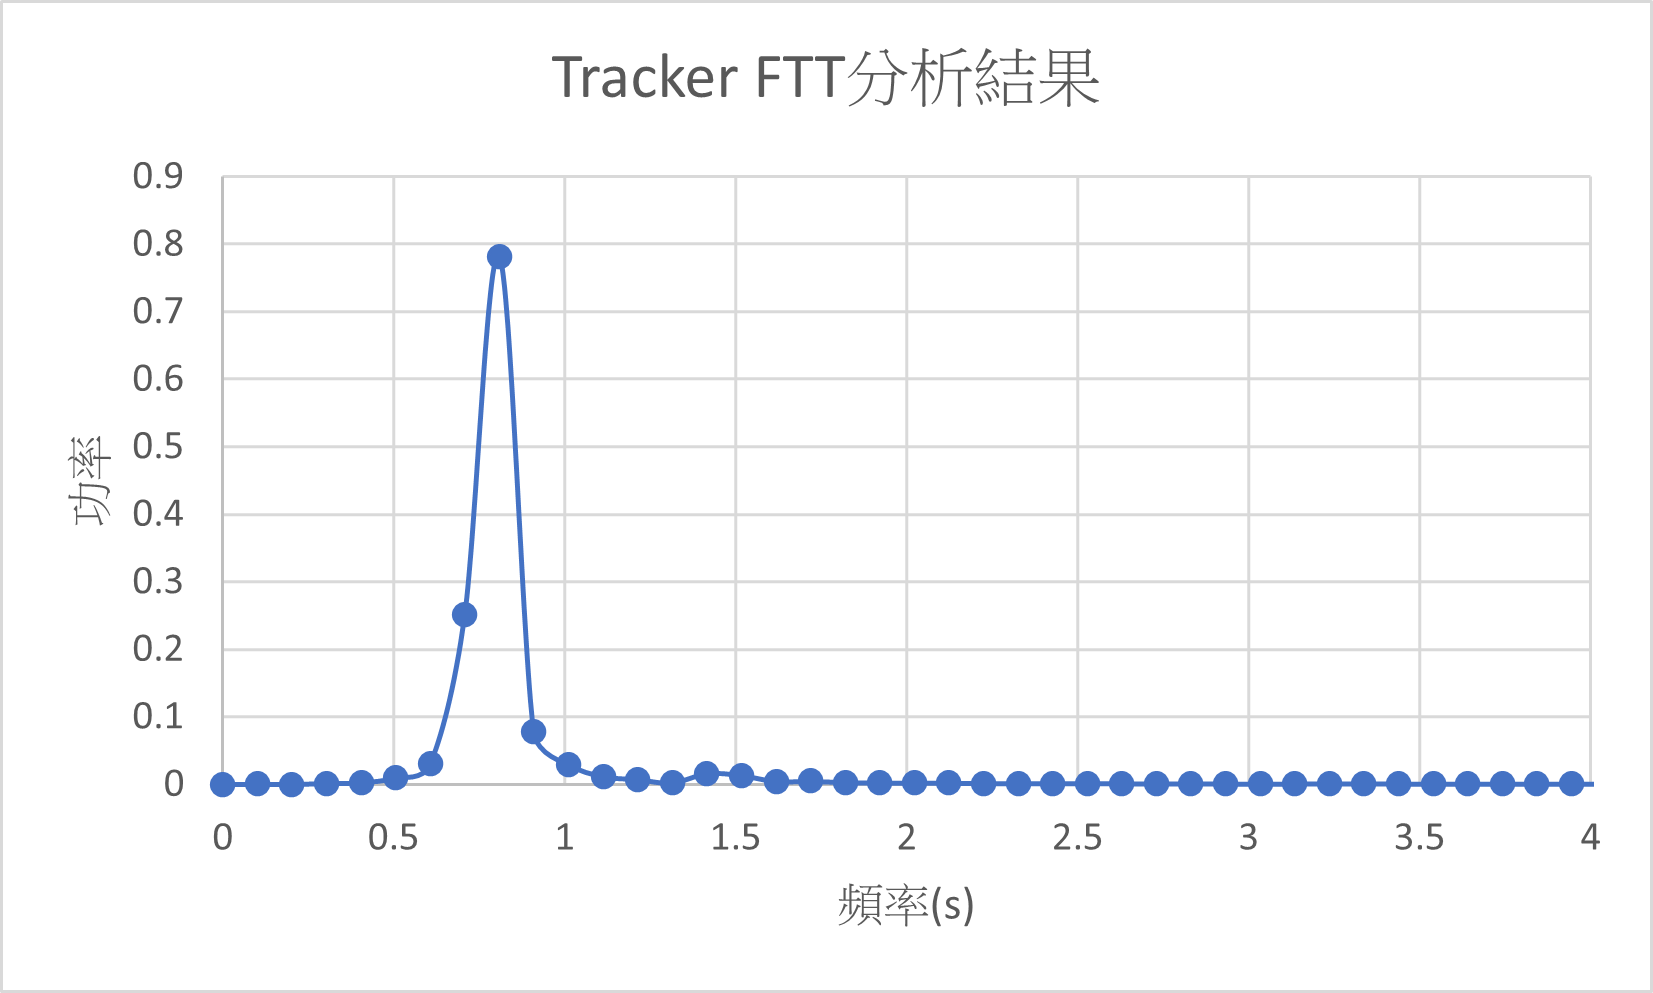
\includegraphics[width=0.7\linewidth]{同向圖表/trackerFTT分析結果.png}
                \caption{trackerFTT分析結果}
                \label{fig:trackerFTT分析結果}
            \end{figure}
            
    \item \textbf{Python擬合結果:}\\
        使用 Python 對實驗數據進行擬合與模擬，可以得到系統的頻率與角速度。擬合結果為：
    \[
    f = 0.9\ \mathrm{Hz}, \quad \omega_p = 5.65\ \mathrm{rad/s}.
    \]
    從圖 \ref{fig:同向震盪pythonFTT模擬圖} 與圖 \ref{fig:同向震盪python模擬} 可以看到，左邊滑車的位移隨時間呈現正弦振盪，且振幅約在 8 秒處歸零，與實驗中測得的振幅衰減趨勢相符。這說明 Python 模擬不僅能擬合振盪週期，也能模擬摩擦力對振幅的影響。  

    此外，Python 模擬提供了完整的數據曲線，便於與實際測量數據對比，觀察實驗誤差來源。例如，雖然頻率略高於 Tracker FFT 與手動計算結果，但整體趨勢吻合，說明 Python 擬合與現實情況差異不大。這也方便後續對不同初始條件或彈簧常數進行分析。
        \begin{figure}[H]
            \centering
            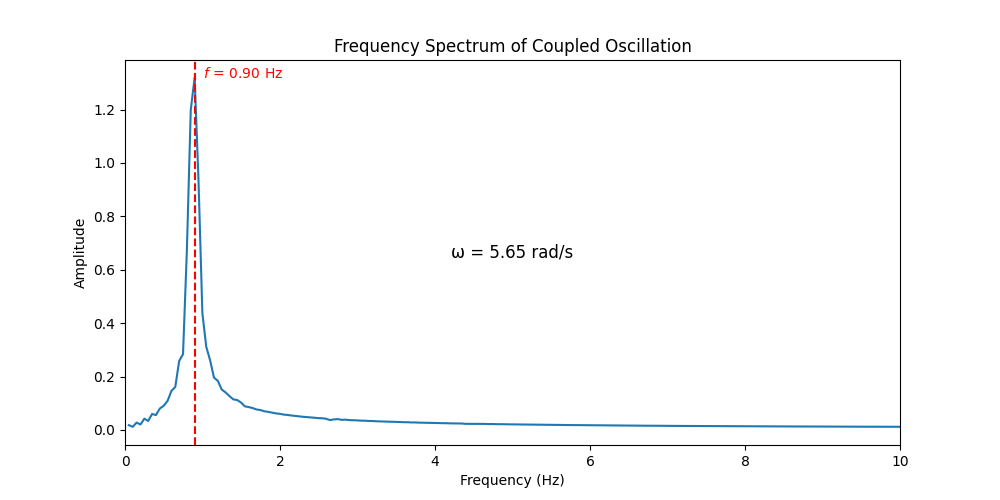
\includegraphics[width=0.85\linewidth]{同向圖表/同向震盪pythonFTT模擬圖.png}
            \caption{同向震盪pythonFTT模擬圖}
            \label{fig:同向震盪pythonFTT模擬圖}
        \end{figure}
        
        \begin{figure}[H]
            \centering
            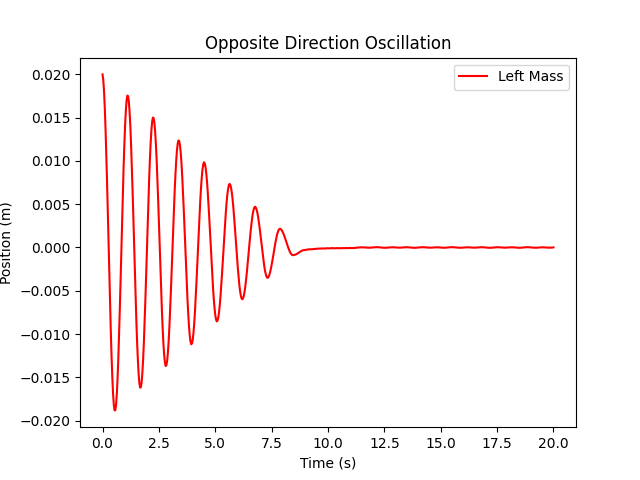
\includegraphics[width=0.7\linewidth]{同向圖表/同向震盪python模擬.png}
            \caption{同向震盪python模擬圖}
            \label{fig:同向震盪python模擬}
        \end{figure}
        
    
    \item \textbf{誤差分析}\\
    將三種方法計算的角速度進行比較：
    \[
    \omega_c = 4.98\ \mathrm{rad/s}, \quad
    \omega_T = 4.98\ \mathrm{rad/s}, \quad
    \omega_p = 5.65\ \mathrm{rad/s}.
    \]
    可以發現，人工計算與 Tracker FFT 的結果幾乎一致，而 Python 模擬的頻率略高，可能原因包括：
    \begin{enumerate}
    \item 手算結果 $\omega_c$ 與 Tracker FFT 結果 $\omega_T$ 幾乎一致，角速度約為 4.98 rad/s，比理論值略低約 10\%。這可能是因為實驗中滑車初始位置測量誤差、彈簧非理想以及摩擦力造成振幅衰減，使得週期變長，角速度變小導致。
    
    \item Python 模擬 $\omega_p$ 考慮了摩擦力，得到角速度 5.65 rad/s，比手算與 Tracker FFT 結果略高，但接近理論值。這說明摩擦力在 Python 模擬中對振幅衰減有影響，但因模擬中的摩擦力為固定值，所以頻率略高於實際測量。
    
    \item 理論值 $\omega$ 為 5.54 rad/s（不考慮摩擦），與 Python 模擬結果差距不大，相對誤差僅約 1.9\%。這說明，摩擦力對週期會產生影響，也會造成振幅衰減。
    \end{enumerate}
    % Please add the following required packages to your document preamble:
    % \usepackage{booktabs}
    \begin{table}[H]
    \centering
    \caption{不同方法計算角速度與理論值比較及誤差分析}
    \label{tab:angular_velocity}
    \begin{tabular}{@{}cccc@{}}
    \toprule
    同向震盪    & 角速度  & 相對Python擬合誤差 & 相對理論誤差 \\ \midrule
    $\omega_c$ & 4.98 & 11.8\%       & 10.1\%  \\
    $\omega_T$ & 4.98 & 11.8\%       & 10.1\% \\
    $\omega_p$ & 5.65 & 0            & 1.9\%  \\
    $\omega$   & 5.54 & 1.9\%        & 0      \\ \bottomrule
    \end{tabular}
    \end{table}
\end{enumerate}
%%%%%%%%%反向
\newpage
\subsubsection{\textbf{反向震盪}}
\noindent
初始位置:$x_1=30cm,x_2=60cm$\\
彈簧變化量:$\Delta x_1=0.03cm,\Delta x_2=-0.03cm$\\
$\omega=\sqrt{\frac{k+2k_{12}}{m}}=9.39\ \mathrm{rad/s}$
\begin{figure}[H]
    \centering
    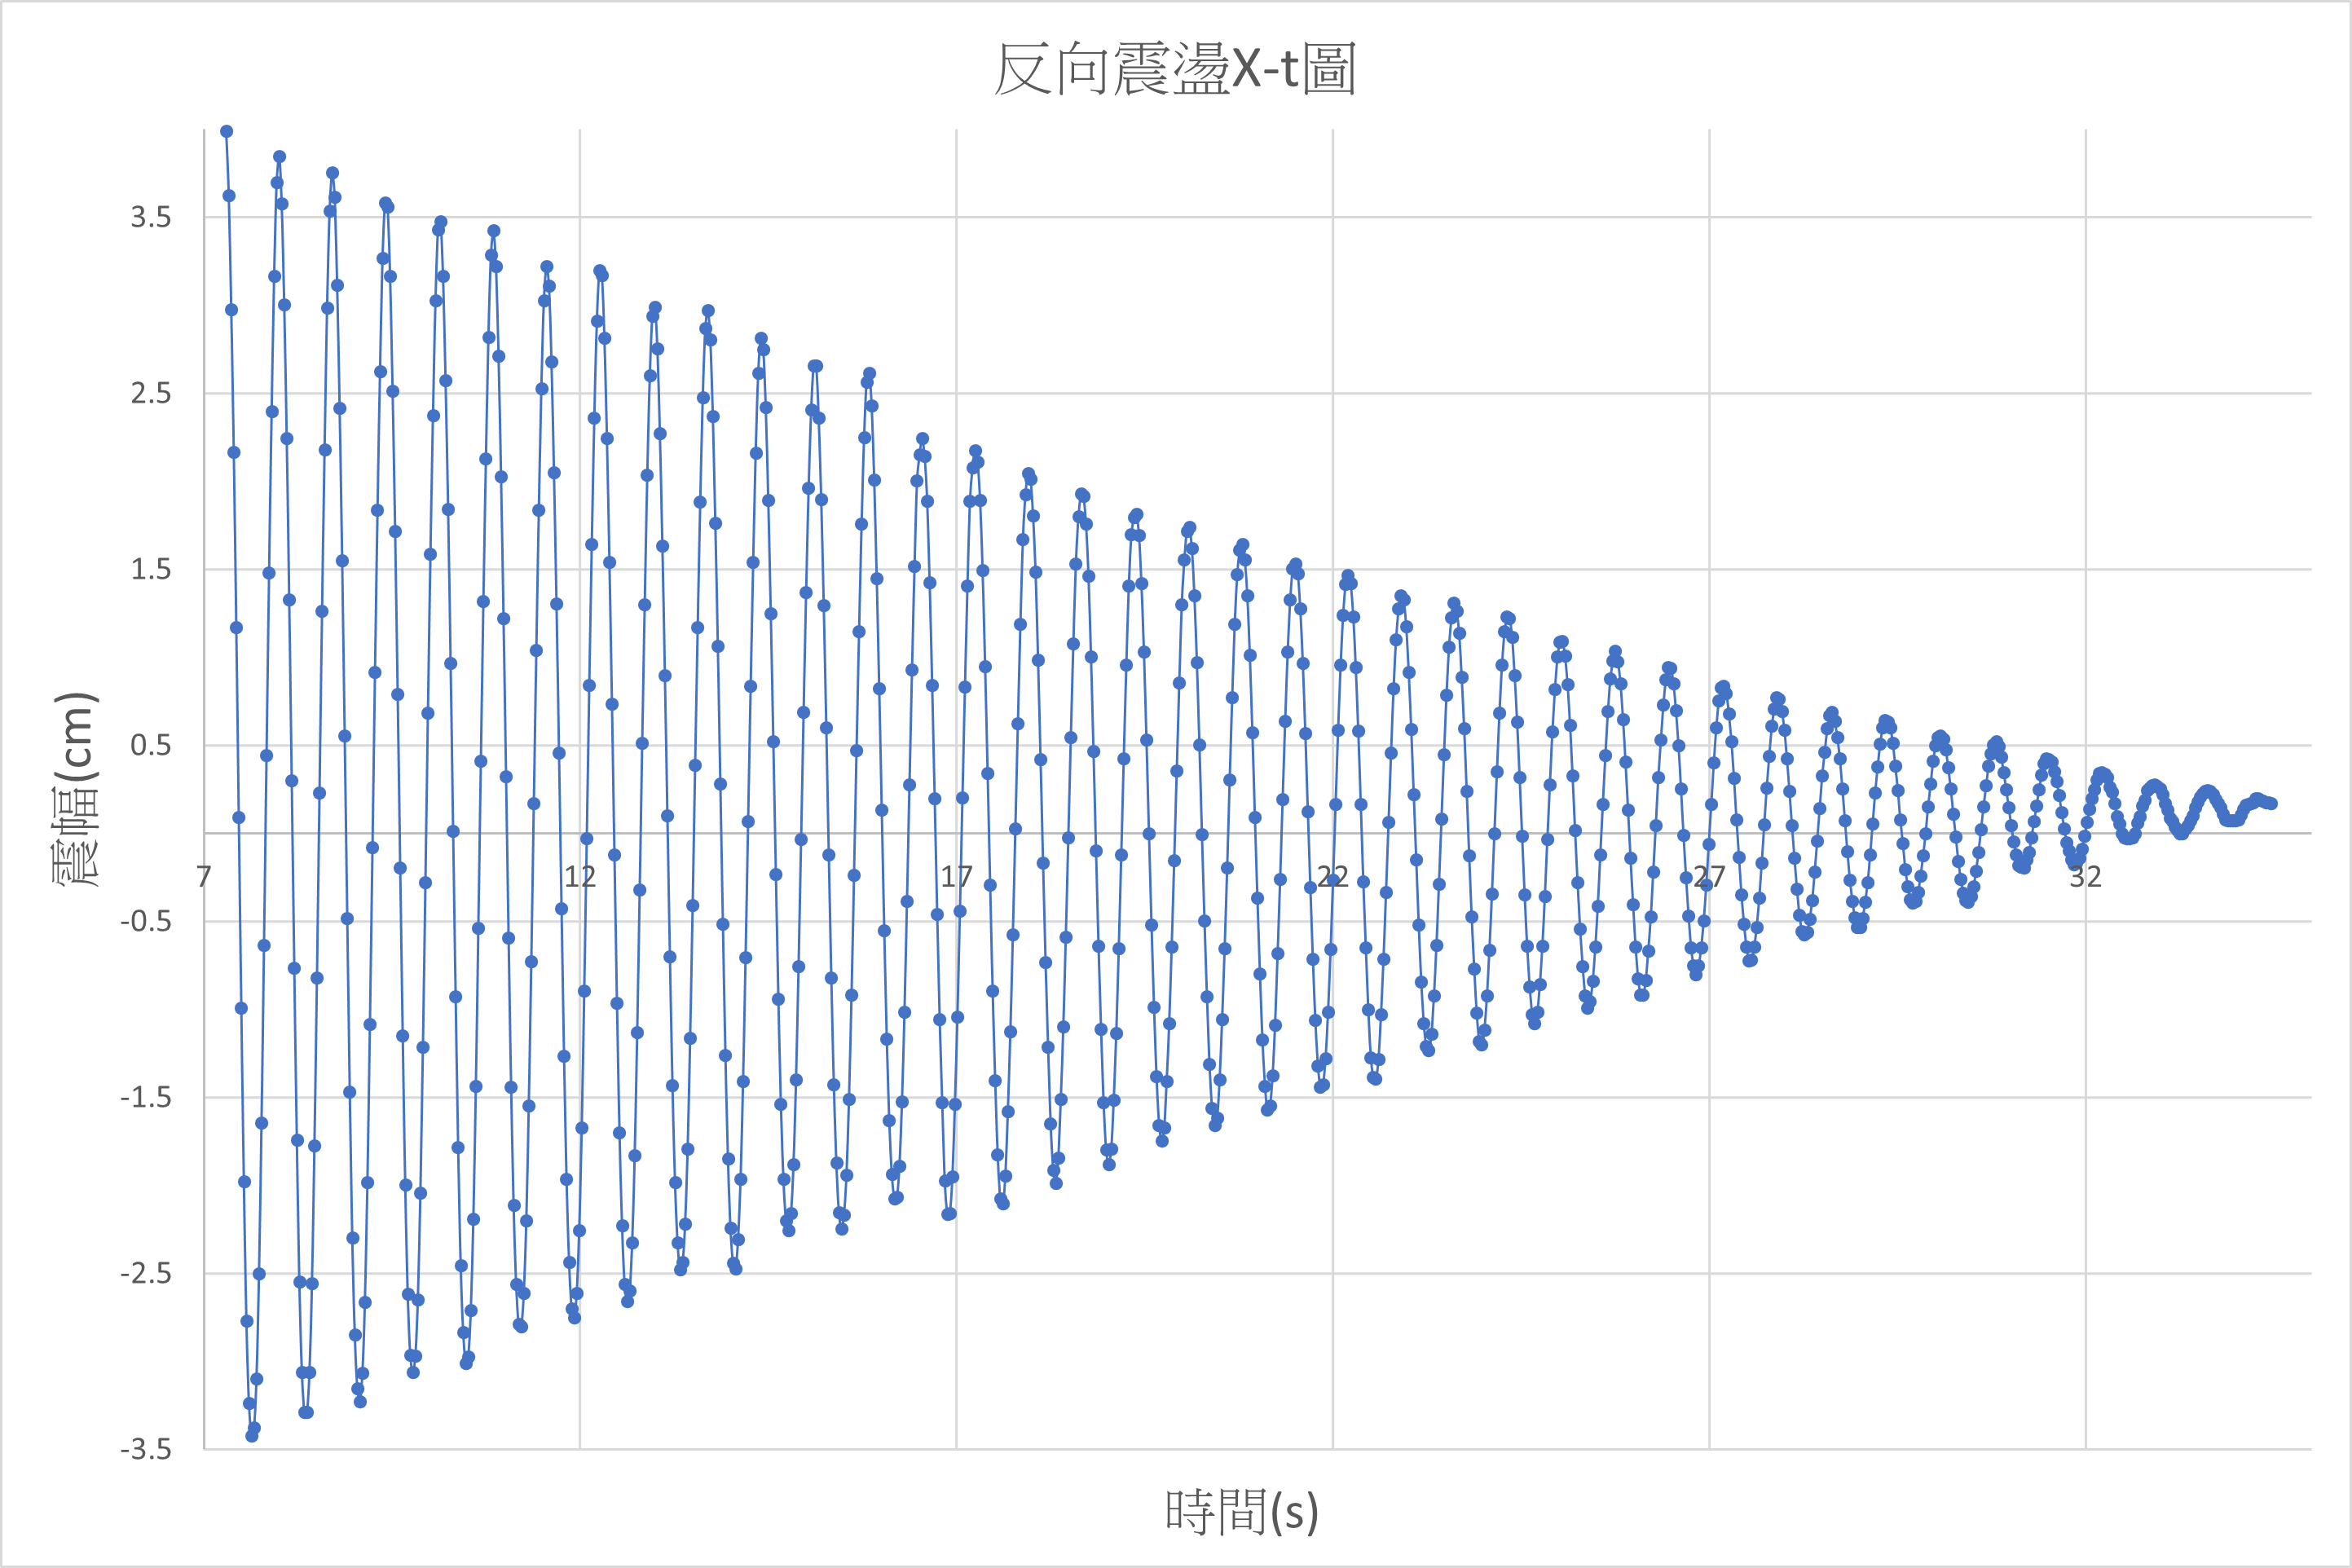
\includegraphics[width=0.7\linewidth]{反向圖表/反向震盪實驗圖.png}
    \caption{反向震盪x-t圖}
    \label{fig:反向震盪xt圖}
\end{figure}
以下我們分別透過 C語言、Traker內建之FTT、python分別對實際實驗數據，擬合結果做分析:
\begin{enumerate}
    \item \textbf{C語言}\\
    透過C計算平均週期後與角速度，結果如圖\ref{fig:反向cprogram分析}所示。
        \begin{figure}[H]
            \centering
            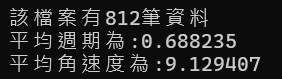
\includegraphics[width=0.5\linewidth]{反向圖表/反向cprogram分析.png}
            \caption{C運行結果}
            \label{fig:反向cprogram分析}
        \end{figure}
        
    \item \textbf{Traker內建之FTT}\\
    使用 Tracker 內建的快速傅立葉轉換（FFT）功能對實驗數據進行頻域分析。分析結果如圖 \ref{fig:反向trackerFTT} 所示。在頻域中，峰值出現在 $f = 1.414$ Hz。根據此頻率，可以計算對應的角速度：
        \[
        \omega_T=2\pi f=8.88\ \mathrm{rad/s}
        \]
        \begin{figure}[H]
            \centering
            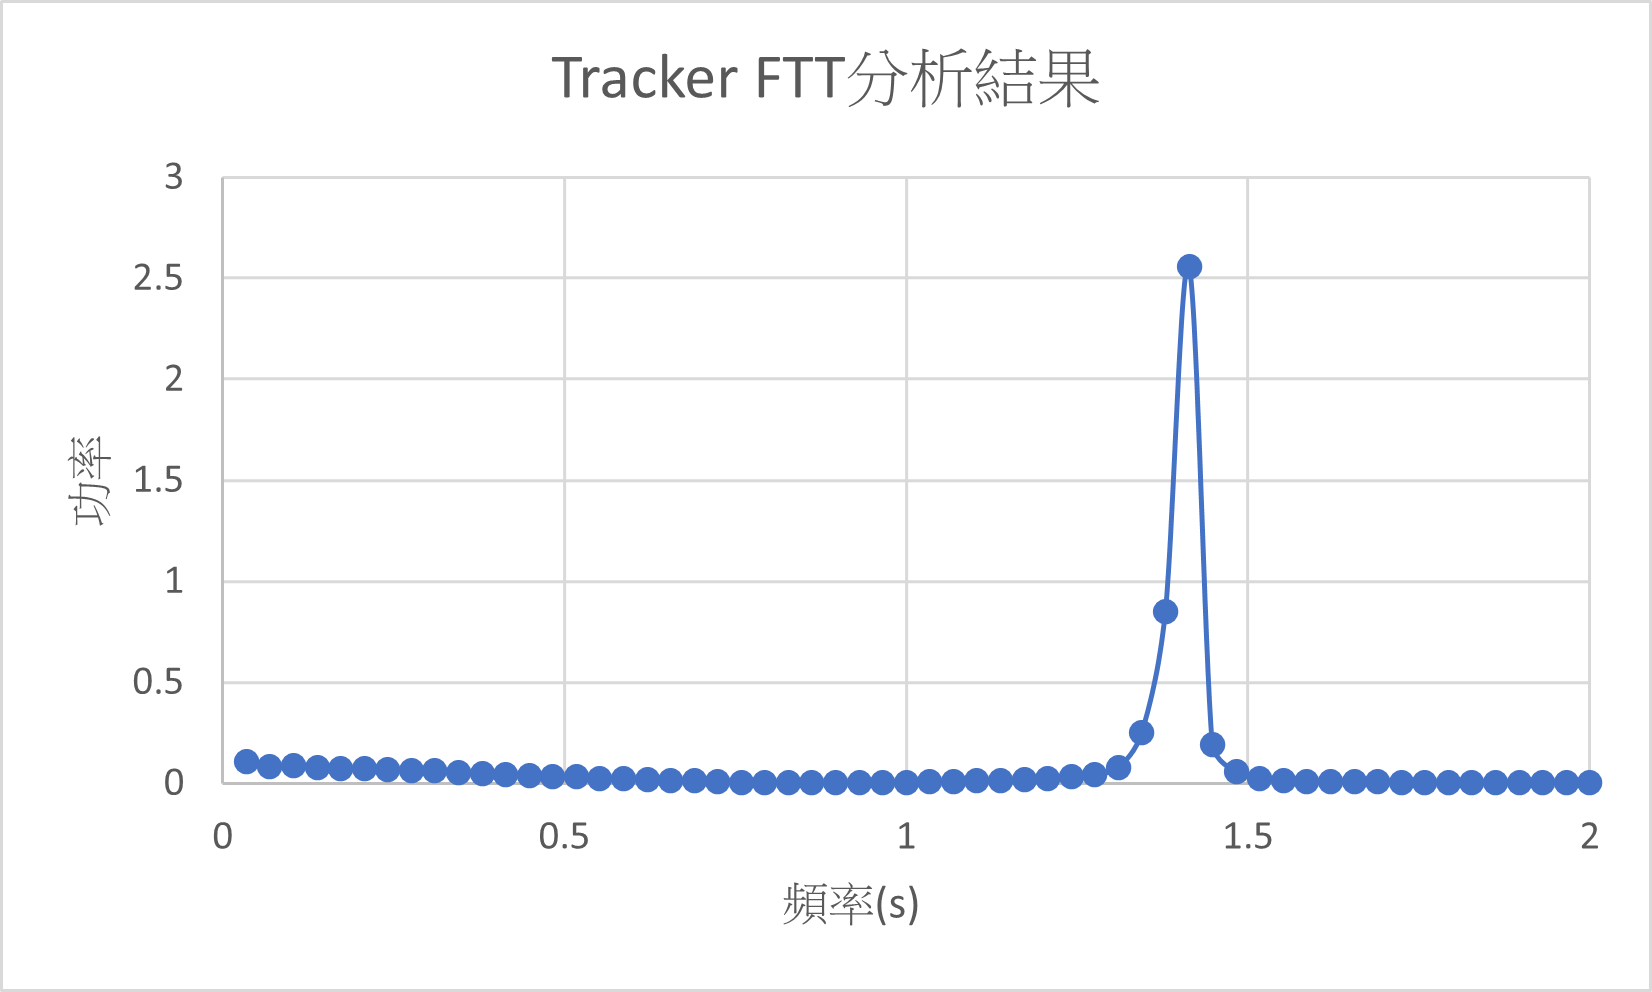
\includegraphics[width=0.7\linewidth]{反向圖表/反向trackerFTT.png}
            \caption{反向trackerFTT}
            \label{fig:反向trackerFTT}
        \end{figure}

    \item \textbf{Python擬合結果:}\\
     使用 Python 對實驗數據進行曲線擬合後，可以取得系統的主要震盪頻率與角速度。程式分析得到：
    \[
    f = 1.50\ \mathrm{Hz},\qquad \omega_p = 9.41\ \mathrm{rad/s}.
    \]

    由圖 \ref{fig:反向python擬合} 與圖 \ref{fig:反向python模擬震盪過程} 可見，模擬中左側滑車的位移與實際量測的振幅衰減相當一致。

    此外，Python 模擬提供完整且連續的時間序列資料，使我們能逐點比較模擬與實驗結果，並檢視可能的誤差來源。雖然 Python 擬合得到的頻率略高於 Tracker FFT 與 C 計算的結果，但整體趨勢仍相符。
        \begin{figure}[H]
            \centering
            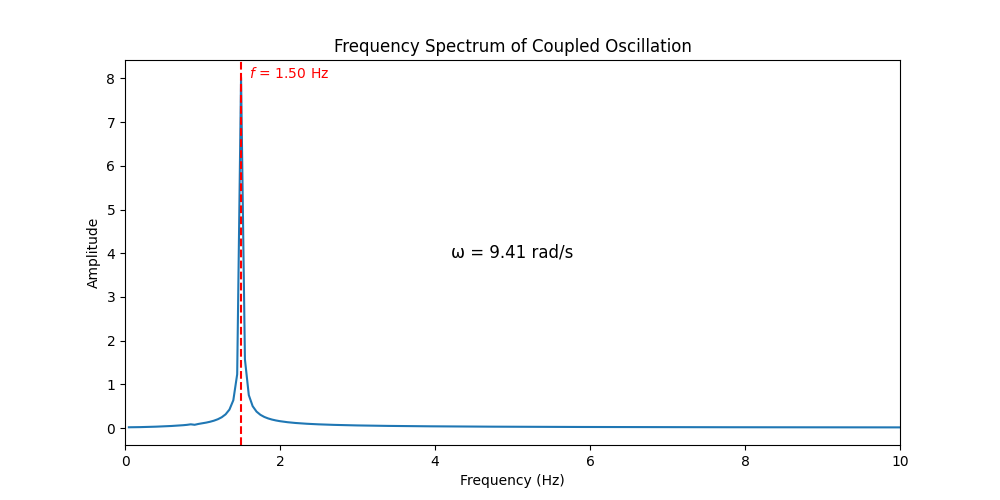
\includegraphics[width=0.7\linewidth]{反向圖表/反向python擬合.png}
            \caption{反向python擬合}
            \label{fig:反向python擬合}
        \end{figure}
        
        \begin{figure}[H]
            \centering
            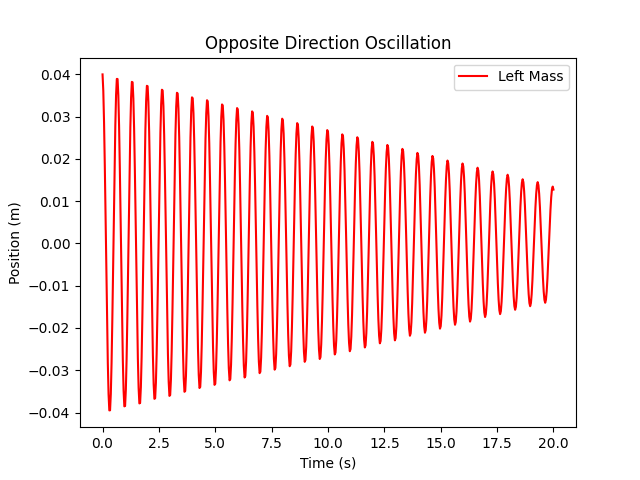
\includegraphics[width=0.7\linewidth]{反向圖表/反向python模擬震盪過程.png}
            \caption{反向python模擬震盪過程}
            \label{fig:反向python模擬震盪過程}
        \end{figure}
        
    \item \textbf{誤差分析}\\
    反向震盪的角速度由三種方法取得，分別為 C 程式計算週期、Tracker FFT 以及 Python 擬合。將三者與理論值
\[
\omega_{\text{theory}}=\sqrt{\frac{k+2k_{12}}{m}}=9.39\ \text{rad/s}
\]
比較後，可以得到以下誤差表（見表 \ref{tab:反向誤差比較}）。

\begin{table}[H]
    \centering
    \caption{不同方法計算角速度與理論值比較及誤差分析}
    \label{tab:反向誤差比較}
    \begin{tabular}{@{}cccc@{}}
    \toprule
    反向震盪    & 角速度  & 相對Python擬合誤差 & 相對理論誤差 \\ \midrule
    $\omega_c$ & 9.13 & 2.9\%       & 2.7\%  \\
    $\omega_T$ & 8.88 & 5.6\%       & 5.4\% \\
    $\omega_p$ & 9.41 & 0           & 0.2\%  \\
    $\omega$   & 9.39 & 0.2\%       & 0      \\ \bottomrule
    \end{tabular}
    \end{table}

由表中可見，\textbf{C 程式的峰值判定法在本次實驗中最接近理論值}，顯示「直接量測週期」的確能得到最準確的角速度估計。其主要原因為反向震盪前期振幅較大，使得峰值容易辨識，因而得到高精度的週期。

誤差來源的比較如下：

\begin{enumerate}
    \item \textbf{C 語言}\\
    利用 C 直接量測相鄰峰值的時間差，因此在振幅足夠的區段能提供極高準確度，並且程式在設計上會自動排除乖離值，讓結果不會失真。並且本次資料的峰值數量充足、雜訊低，因此使用 C 誤差最小，為最準確的方法。

    \item \textbf{Tracker FFT 的誤差來源}\\
    在FTT分析時，tracker會計算到快結束時的震盪，而這些震盪的波型經常是不規則的，所以使頻率失真。在此實驗中，震盪末期的週期漸漸變大(如圖\ref{fig:反向震盪波型})，這也讓得出的角速度偏小。
    \begin{figure}[H]
    \centering

    \begin{subfigure}{0.45\textwidth}
        \centering
        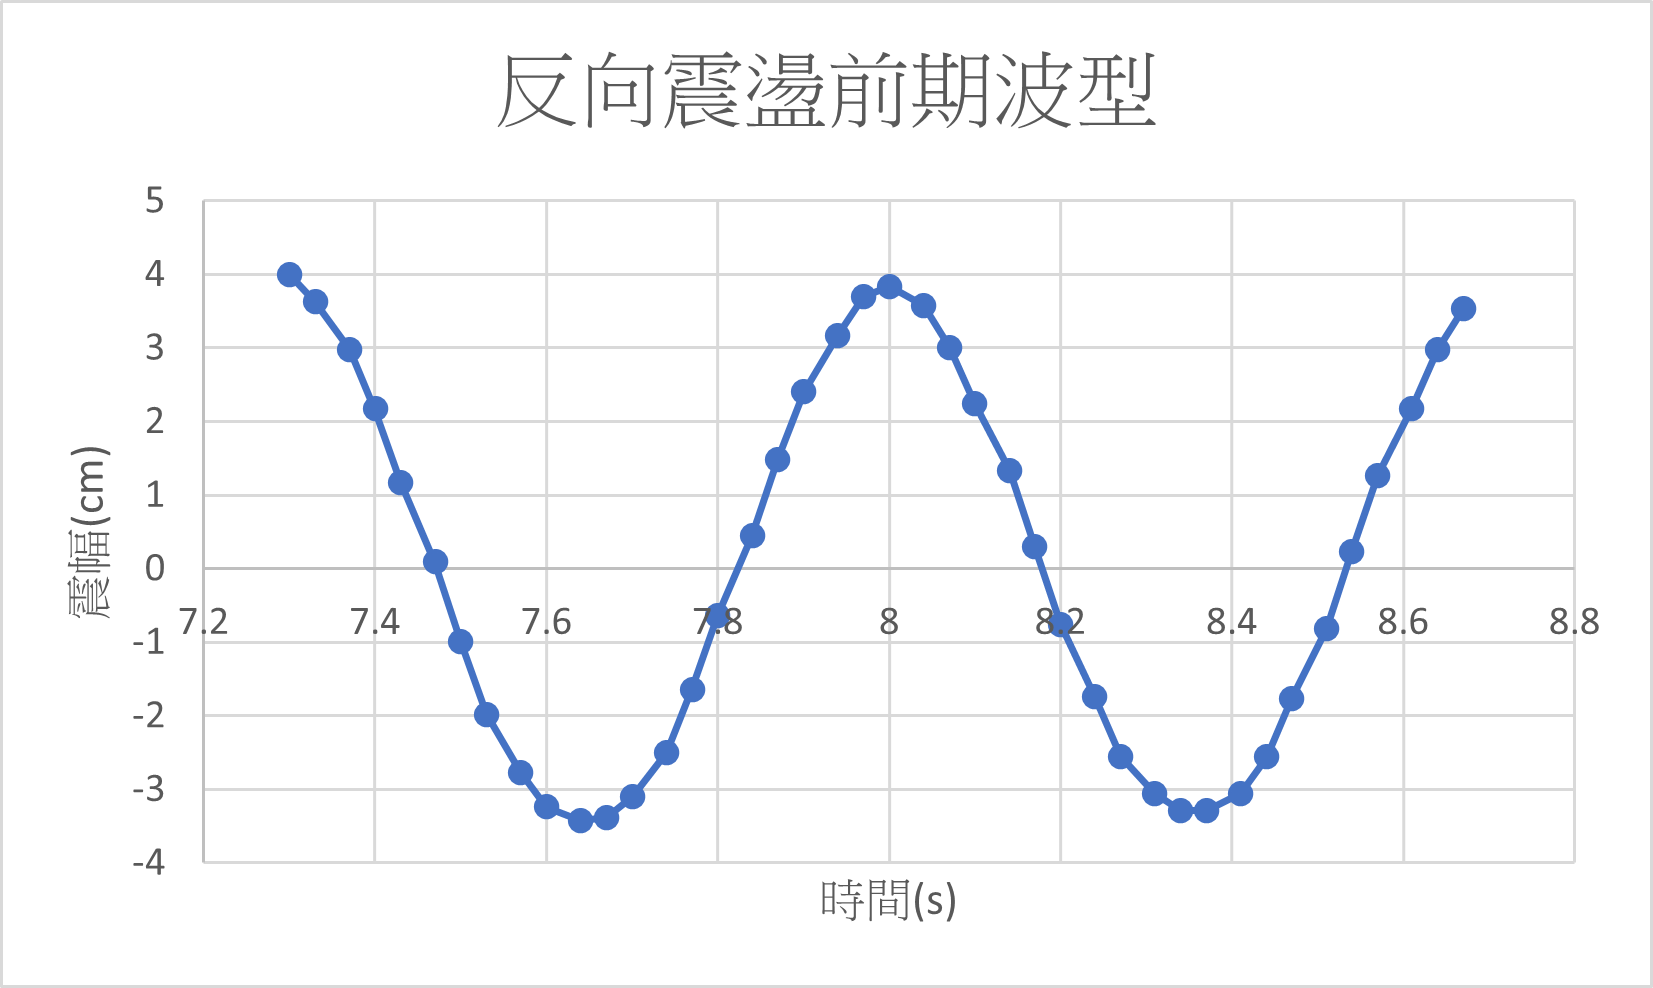
\includegraphics[width=\linewidth]{反向圖表/前期圖片.png}
        \caption{前期}
        \label{fig:subfig1}
    \end{subfigure}
    \hfill
    \begin{subfigure}{0.45\textwidth}
        \centering
        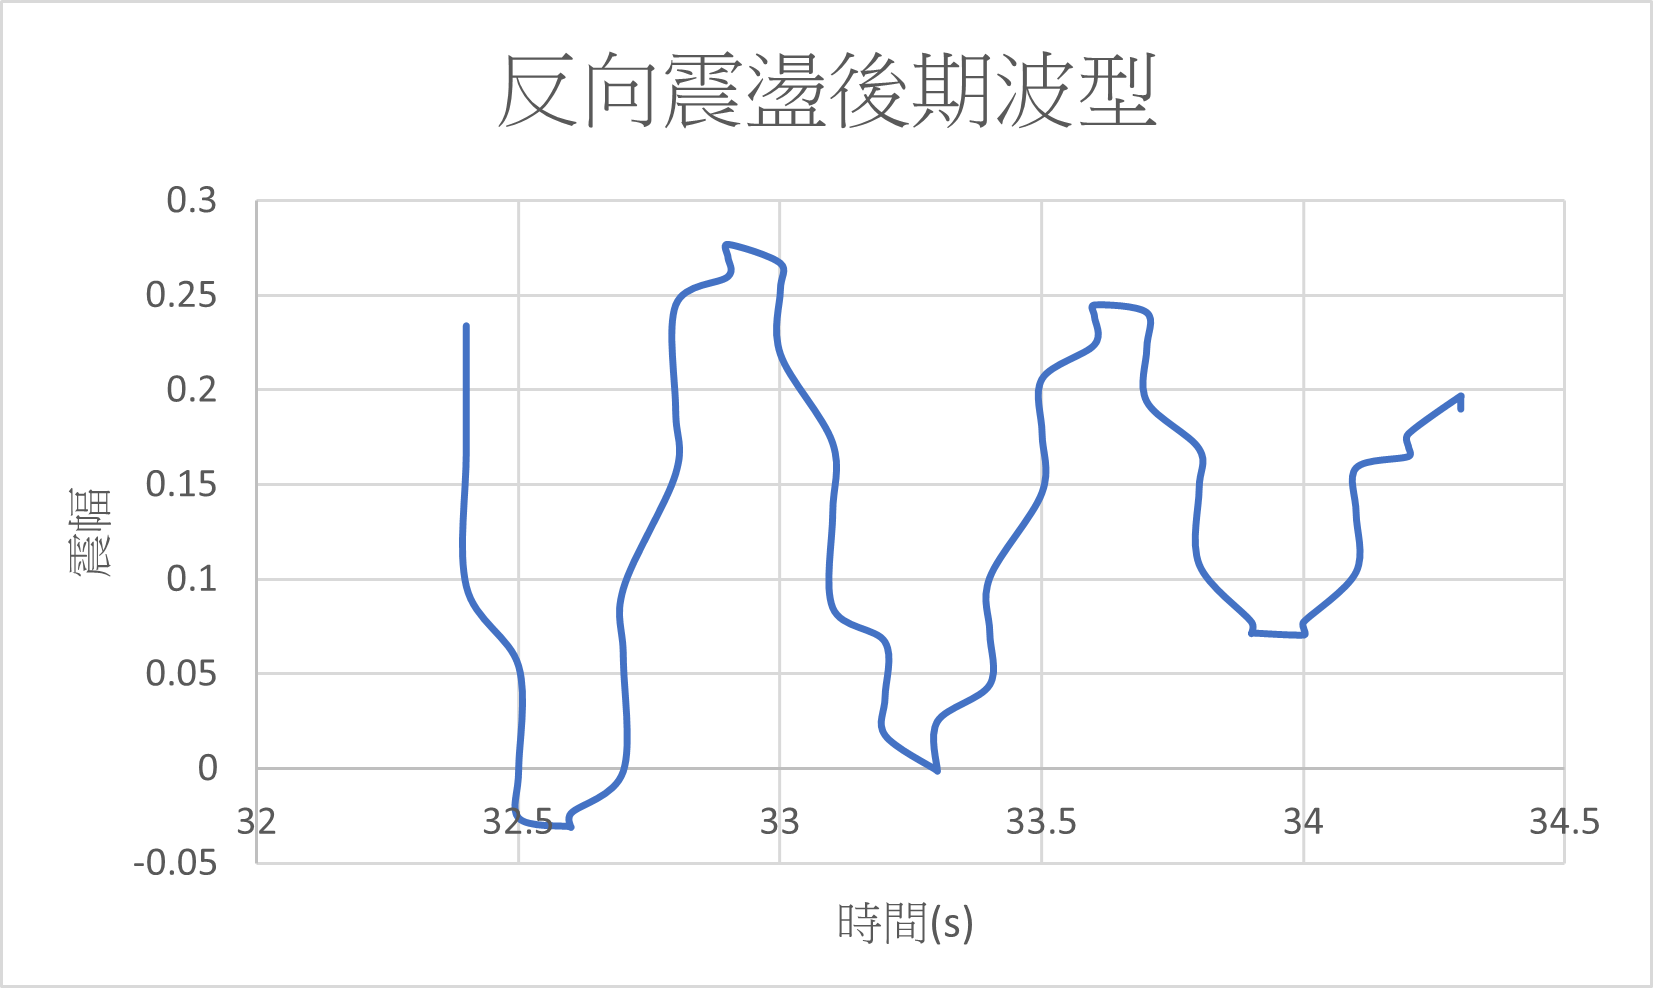
\includegraphics[width=\linewidth]{反向圖表/後期圖片.png}
        \caption{後期}
        \label{fig:subfig2}
    \end{subfigure}

    \caption{反向震盪波型}
    \label{fig:反向震盪波型}
    \end{figure}
\end{enumerate}
\end{enumerate}
%%%%%%%%%%%%%%%%%%%%%%%%%%%%%%%%%%%%%%%%%%%%%%%%%%%%%%%%%%%%%%%%
\section{\textbf{結果與討論}}
實驗結果顯示，同向與反向震盪的角速度與理論值大致吻合。從 Tracker 與 Python 擬合曲線可觀察到，反向震盪的振幅衰減較快，主要原因為摩擦力作用所導致。\\
整體而言，三種方法（C程式、Tracker FFT、Python擬合）皆能有效處理系統特徵頻率，誤差控制在 10\% 以內。此結果驗證了耦合振盪系統的模態分析理論，並顯示初始條件對振幅分布的影響。
%%%%%%%%%%%%%%%%%%%%%%%%%%%%%%%%%%%%%%%%%%%%%%%%%%%%%%%%%%%%
\newpage
\section{\textbf{思考問題}}
%%%%%%%%%%%%%%%%%%%%%%%%%%%%%%%%%%%%%%%%%%%%%%%%%%%%%%%%%%%%%
\textbf{1. 在某些初始條件的設定之下，會發現滑車的振盪幅度有變大變小的情況。為什麼?
}

\noindent
------------------------------------------------------------------------------------------------------

This phenomenon is called \textbf{beating }in coupled oscillators.

→  When you have two modes, with slightly different frequency and initial conditions, sometimes the modes will have a chance to \textbf{subtract} themselves from each other, causing the total amplitude to sometimes jump up and down.


→e.g: $x(t)=A_1\cos(\omega_1t)+A_2\cos(\omega_2t)$

{\small If $\omega_2>\omega_1$, there’s a possibility when $A_1\cos{(\omega_1t)}>A_2\cos{(\omega_2t)}$ , and with some values, the value could become negative.}

\noindent
------------------------------------------------------------------------------------------------------

   
\textbf{2. 數值方法中的Euler method是否能讓總能量守恆？}

\noindent
------------------------------------------------------------------------------------------------------

No. It is not energy conserving. The Euler method:
\[ x_{n+1}=x_n+v_n \Delta t\]
\[ v_{n+1}=v_n+a_n \Delta t\]

{\small 
Note: $x$ is distance, $v$ is velocity, and $a$ is acceleration.}

\vspace{0.5cm}
Has a fatal \textbf{disadvantage} of being error accumulating. Every little error tends to build up one by one, resulting in a visible difference in data output.

%%%%%%%%%%%%%%%%%%%%%%%%%%%%%%%%%%%%%%%%%%%%%%%%%%%%%%%%%%%%%%%%5
\noindent
------------------------------------------------------------------------------------------------------
\newpage
\section{附錄:程式}

\begin{lstlisting}[language=C, caption={找出資料峰值，計算週期}]
#include<stdio.h>
#include <stdlib.h>
#include <math.h>

int main(void)
{
	char filename[100];
    scanf("%s",&filename);
	FILE *fp=fopen(filename,"r");//開啟檔案
	if(fp==NULL)
	{
		printf("沒有該檔案");
		return 1;
	}
	//讀取資料 
	double time[1500],x_axis[1500];
	int i=0;
	while(fscanf(fp,"%lf,%lf",&time[i],&x_axis[i])==2)
	{
		i++;
		if(i>=1500)	break;
	}
	fclose(fp);
	printf("該檔案有%d筆資料\n",i);
	//找高峰 
	double peak_time[1500];
	int peak_count=0,j=1;
	for(;j<i;j++)
	{
		if(x_axis[j] > x_axis[j-1] && x_axis[j] > x_axis[j+1])
		{
			peak_time[peak_count]=time[j];
			peak_count++;
		}
	}
	if(peak_count<2) 
	{
		printf("無法計算週期\n");
		return 1;
	}
    
	//計算週期 
	double period[1500];
	int period_count=0,k=1;
	
	for(;k < peak_count;k++)
	{
		if( peak_time[k]-peak_time[k-1] <=1 )
		{
			period[period_count]=peak_time[k]-peak_time[k-1]; 
			period_count++;
		}
	}
	
	//平均週期
	double sumT=0,Tavg=0,omega=0;
	for(i=0; i< period_count;i++) 
	{
		sumT+=period[i];
	}
	
	Tavg=sumT/period_count;
	omega=(2*3.14159)/Tavg;
	
	printf("平均週期為:%lf\n",Tavg);
	printf("平均角速度為:%lf",omega);
	
	return 0;

 }

\end{lstlisting}

\end{document}